\documentclass[11pt,DIV12,BCOR0mm,oneside,headings=normal,%
  numbers=noenddot,headsepline,headinclude]{scrreprt}
\usepackage[automark,headsepline]{scrpage2}
\usepackage{scrhack}                % to avoid KOMA-Script warning
\usepackage[utf8]{inputenc}         % UTF8 encoding
%\usepackage[latin1]{inputenc}      % ISO encoding
\usepackage[T1]{fontenc}
\usepackage{txfonts}                % Postscript fonts
\usepackage[ngerman,english]{babel}
\usepackage[fixlanguage]{babelbib}
\usepackage{graphicx}
\usepackage[usenames]{xcolor}
\usepackage{listings}
\usepackage[pdftex]{hyperref}       % provides \url
\usepackage{wallpaper}              % for HsH logo
\usepackage{subfigure}


% ---------------------------------------------------------

% package configuration
\KOMAoptions{headinclude}       % for scrpage2
\lstset{numbers=none,showstringspaces=false,language=Java,%
  basicstyle=\ttfamily,frame=single,rulecolor=\color{gray}}
\hypersetup{linkcolor=black,pdfborder=0 0 0}

% layout
\tolerance=2000                 % avoid overfull hboxes
\frenchspacing                  % no extra space after full stops

% ---------------------------------------------------------

\begin{document}

\selectlanguage{english}
\selectbiblanguage{english}

% title page
\thispagestyle{empty}
%\cleardoublepage
\pagenumbering{roman}

\begin{center}
  \vspace*{4\baselineskip}
  {\sffamily\bfseries\LARGE
    Redis Database Analyses\par}
  
  \vspace*{4\baselineskip}
  {\Large }

  \vfill
  {\Large }
  \begin{figure}[htb!]
  	\centerline{
\includegraphics[width=0.8\textwidth]{resources/Redis_Logo.png}}
  \end{figure}
  
  
  \vspace*{4\baselineskip}
  {\Large \par}
  
  \vspace*{4\baselineskip}
  {\Large 20.\,10.\,2016}
  
  \vspace*{4\baselineskip}
\end{center}


{\huge\textbf{Written by}} \\
\\
\\
\textbf{} \\
Florian Sander \\
florian.sander@student.hs-hannover.de \\
\\
\\
\textbf{} \\
Nikolai Böker \\
nikolai.boeker@student.hs-hannover.de \\
\\
\\
\textbf{} \\
Danar Armin \\
danaramin5889@gmail.com \\
\\
\\
\textbf{} \\
Sana Lakhal \\
sana.lakhal@student.hs-hannover.de \\
\\
\\
\textbf{} \\
Sascha Becker \\
s.becker@wertarbyte.com \\
\\
\\
\\
\\


\tableofcontents    % Table of Contents

%\listoftables       % Tabellenverzeichnis

% main text
\newpage
\pagenumbering{arabic}
\chapter{Data Model}

Redis is a NoSQL database with an aggregate orientation and is likewise key-based \cite{redis} \cite{redis_book}. This means that keys identify the assigned value, this way a client can extract the value by knowing its key. Further you can put a value for a key or delete a key and likewise its value. Redis keys are binary safe which means any binary sequence can be used as a key. An empty string is also a valid key. But Redis is not a plain key-value store. Because a key is binary safe the value can hold more complex data structures. By complex is meant the possibility to nest values in values or even map objects. 

\section{Data Structures}
Redis supports the following data structures:
\begin{itemize}  
\item Strings: a String-value can have a total length of 512 Mb, assembling Strings
\item Lists: simply an ordered list of Strings => a sequence with duplicates, adding 	new elements on the head (left) or on the tail (right), max length of a list is 232 (around 4 billion of elements per list
\item Hashes: maps between String-fields and String-values, mainly represent objects, have a max length of 232
\item Sets: an ordered collection of Strings, not allowing duplicates (if u add the 	same element multiple times will result in having just a single copy of this element), max number of elements is the same as lists, you can apply commands or set operations
\item Sorted Sets: similar to Set but associated with a score ordering the sorted set from the smallest to the greatest score, elements are unique but scores may be repeated
\item Bitmaps and HyperLogLogs: basing on Strings with their own semantic Message Queues 	
\end{itemize}

You can run atomic operations on each of these data types. With SET you set a specific value for a key and with GET you retrieve this value. SET replaces any existing value already stored into a key in the case this key already exists. This way SET can be used to update a value of an existing key. Because the value of the key is overwritten with a new value, the old value is kind of deleted. To delete a key with its associated value you run the command DEL. Redis offers the possibility to set or retrieve the value of multiple keys in a single command using MSET and MGET. MGET returns an array of values.

Redis supports around 50 programing languages. 12 languages are particular recommended. For Java there are 4 different libraries. A few examples for different programming languages in the following are JRedis for Java , Redis-rb for Ruby, Credis for C and Redis-py for Python.
\chapter{Query Support}

\section{Types}
Redis supports different query types. Redis supports point and range queries for:
strings, hashes, lists, sets, sorted sets. A string for example can be accesses via GET <key> and multiple Strings can be accesses, to name one possibility, for example with the command: MGET <key> [<key>…]. Geospatial indexes can even be searched by radius queries. That means Redis checks if the geospatial indexes are within a specific radius of a defined
position. Arbitrary access of entries is also possible by getting a random key with the command RANDOMKEY. In comparison to plain key-value stores, redis is able to store complex data structures and perform for the data structure specific commands. So for example in redis it is possible in a list to prepend one or multiple values with the command: LPUSH <key> <value> [<value>…]. Another mentionable functionality of redis is that keys can expire. Timeouts can be set on keys and after the timeout has expired, the key will automatically be deleted. The related command for expiring a key is the command: EXPIRE <key> {seconds}.

\section{Language}
In comparison to normal SQL Redis doesn‘t have a delarative query language. The query language of Redis is imperative. All queries in Redis are made with commands that can‘t be modified (apart from source code modifications in Ansi-C), except for the arguments, that can be passed into the command.

\section{Are queries automatically optimized?}
There is no automatic command optimization in Redis. One comparable approach in Redis is the Slowlog. Redis logs queries that exceed a specific, configurable execution time. The execution time is just the time actually needed to execute the command, not included in this case are for example the I/O operations or the communication with the client. With the Slowlog there is a chance to identify slowly executing commands. The commands themselfs aren‘t automatically optimized.

\chapter{Indexes}

In Redis different kinds of indexes can be created. The following indexes can be created using sorted sets:

\section{Simple Numerical Indexes}
\begin{itemize}
\item Simplest index that can be created in Redis
\item Numerical value can be indexed
\item Data type of sorted set is used which represents a set of elements
\item Elements are ordered by a so-called score
\item Scores are in ascending order
\item Updating this kind of index must be done manually
\begin{itemize}
\item Adding back again an element with a different score and the same value
\item Two operations (commands) needed:
\begin{enumerate}
\item Updating the data in the hash that representing the element    (HSET)
\item Updating the data in the index (ZADD)
\end{enumerate}
\end{itemize}
\end{itemize}

\section{Lexicographical Indexes}
\begin{itemize}
\item In Redis when elements with the same score are added into a sorted set, then they are ordered lexicographically
\item Strings are indexed
\begin{itemize}
\item Strings are compared as binary data
\item Elements are sorted by the raw values of their bytes (byte after byte)
\end{itemize}
\item Lexicographical indexes are managed manually
\begin{itemize}
\item One possibility to update index values is to take a hash in addition to    the sorted set; the hash maps the object ID to the current index value
\item In case of removing old information were indexed the hash value   has to be retrieved by object ID and then the information can be removed from the sorted set (command: ZREM)
\end{itemize}
\end{itemize}

\section{Composite Indexes}
\begin{itemize}
\item Are used when indexes are created by using multiple fields
\item Composite indexes can also be used in order to represent graphs by using the so-called Hexastore data structure
\begin{itemize}
\item By using Hexastore relations between objects can be represented
\item An element (relation) must be stored in a lexicographical index
\end{itemize}
\end{itemize}





\chapter{Persistence}
Redis comes with a different range of options when it comes to persistence \cite{redis_persistence}. 

\section{RDB}
The RDB persistence performs point-in-time snapshots of your dataset at specified intervals.
Due to its compact size it is perfect for backups. Store those single files on a separate server or in the cloud e.g. Amazon S3.
In case of a disaster you can easily restore a different version of the data set.
Restarting your service with RDB will be faster since it is only a single file that must be loaded.

On the downside you have to live with data being lost when restoring a state. Due to the RDB timed saving interval mechanic data missing a save point will be lost once something bad happens.
To reduce the amount of data being lost minimizing the time interval will create backups more frequently.
Everytime RDB has to persist something on the disk it is using a child process and starts to fork(). This can be time consuming if you are working with a big dataset.

\subsection{Snapshotting}
So called „in-memory“ meaning Redis holds the „Dictionary“ in the RAM and stores it onto the disk at predetermined intervals. The intervals to store data onto the disk can be configured by define the number of writing operations and a time limit.If the systems crushes the past operations can be reloaded to retrieve the primary state of the data.

\section{AOF}
Instead of saving a complete dataset AOF logs your actions and reconstruct your dataset when started.
This log is append only which prevents corruption problems if there is a power outage. If the log contains a half written action the provided redis-check-aof tool will be able to fix that.
The log will grow for sure. Every action will be appended. To prevent a big log file Redis will rewrite it frequently. AOF will minimize the amount of actions needed to restore your dataset. If the second file is ready refactoring it will switch it with the original and starts appending onto the new one.
Further more the log file is human readable. In case of a disaster you can check the log for problems and edit them directly. Restart and AOF will use your edited lines.

On the downside the AOF files are usually bigger than a RDB file for the same dataset. Depending on the used fsync policy AOF can be slower than RDB.

\subsection{Append-only file}
Every writing operation is stored onto the disk immediately.

\section{Combine AOF and RDB}
You can combine those two options for a hybrid solution. In this scenario Redis will use the AOF file when restarting to reconstruct the original dataset because it is the most complete.

\section{No persistence}
If you are risky disable persistence completely. Just use Redis as is. There will be no backup or restoring features with this option.

\section{What's the best option now?}
It depends on your requirements If you want a degree of data security comparable to what postgreSQL provides choose the hybrid option.
If your data is very delicate but living with a few minutes of data loss is acceptable choose RDB alone.
Choosing AOF alone is something you should prevent. Taking a RDB snapshot form time to time is a must have if you seek for backups.
\chapter{Transactions and Concurrency Control}

Redis support transactions. A basic transaction is a sequence of multiple commands. One client can execute multiple commands without other clients being able to interrupt them \cite{redis_labs_transactions}. In Redis the foundation of transactions are following commands: MULTI, EXEC, DISCARD and WATCH, which allow execution of a group of commands in a single step. The basic usage is to enter MULTI, enter multiple queries and enter EXEC for executing the multiple commands or  DISCARD for flushing the transaction queue. Every command passed as a part of a basic MULTI/EXEC transaction is executed one after another until they have completed. After completion another client may execute their commands. The WATCH command is used to provide a check-and-set behavior to transactions. This form of locking is called optimistic locking (which is an Optimistic Concurrency Control, short: OCC approach).

\section{Transaction guarantees}
\begin{itemize}
	\item All commands in a transaction are serialized no request by other client is served in the middle of the execution of a Redis Transaction guarantees isolation
	\item All commands are processed or none guarantees atomic transactions
\end{itemize}

\section{Errors}
A possible error before a transaction could be that the command maybe failed to queue due to wrong syntax of the command or e.g. memory errors. Another eventuality to produce an error after a transaction is executed could be to execute a command against a key with a wrong data structure (all data structures have specific commands and the actual values are unknown for the system). Even though a command might fail during execution, the execution of the following commands will be processed and not rolled back like in some relative database query languages \cite{redis_transactions}.

\section{PCC}
Pessimistic Concurrency Controls (PCC) in distributed systems, with distributed locks are also possible with Redis, but not with the commands in the Redis query language itself. If necessary, the “Redlock” algorithm can be integrated in diverse programming languages.

\chapter{Partitioning}

Splitting Redis into multiple instances is a process called partitioning. Every instance will only contain a small subset of the keys.

Partitioning servers two main goals:
\begin{itemize}
	\item The Database can be much larger because using multiple computers merged into one is more powerful than using a single instance
	\item Scaling becomes reality. Giving control over how much cores and instances used in your cluster is a must for bigger systems
\end{itemize}

\section{Types}
There are several ways to split up your keys and route your users to what they need.

\subsection{Range Partitioning}
As the name suggests you define ranges of object into specific Redis instances. This system requires a table that maps ranges to instances. It needs to be managed and it's needed for every kind of object. Because of that it's much more inefficient than other methods.
\subsection{Hash Partitioning}
An alternative is hash partitioning. This method just needs a key. The process is as follows:
\begin{itemize}
	\item Hash the key to turn it into a number e.g. with the crc32 hash function
	\item Using modulo on this number and turn it into a number between 0 and n-1. Where n is my number of available Redis instances
\end{itemize}

\section{Where and how implemented?}
The responsibility can be part of different parts of a software stack
\begin{itemize}
	\item Client side partitioning pushes the responsibility choosing a fitting node to the client
	\item Proxy assisted partitioning adds a proxy layer between the client and a Redis node. It chooses the right one for you
	\item Query routing allows sending to any instance and choosing the right one for you
\end{itemize}

\section{Disadvantages}
Everything can't be gold so there has to be some problems.
\begin{itemize}
	\item Operations that need multiple sets on different instances are not possible
	\item Transactions involving multiple keys cannot be used
	\item Backup and logging (RDB and AOF) becomes more complex because it has to done for every instance
\end{itemize}
\chapter{Platform}
Redis is written in ANSI C and works in most POSIX systems like Linux, *BSD, OS X without external dependencies. Linux and OS X are the two operating systems where Redis is developed and more tested, and we recommend using Linux for deploying. Redis may work in Solaris-derived systems like SmartOS, but the support is best effort. There is no official support for Windows builds, but Microsoft develops and maintains a Win-64 port of Redis.

\section{Run Redis on Google Cloud Platform}
Redis is an open source (BSD licensed), in-memory data structure store, used as database, cache and message broker.
It's easy to get started developing Redis apps running on Google Cloud Platform. And because the apps you create will be running on the same infrastructure that powers all of Google's products, you can be confident that they will scale to serve all of your users, whether there are a few or millions of them.

The following diagram shows the process of deploying the app on Cloud Platform.

\begin{figure}[htb!]
\centerline{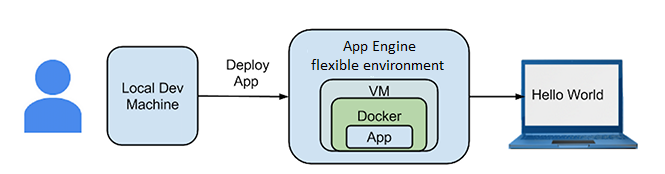
\includegraphics{resources/hello-world-app-structure.png}}
\caption{Hello World App Structure}
\label{hello-world-app-structure}
\end{figure}
The App Engine flexible environment runs your application in containers that can automatically scale to handle your application's load. Behind the scenes, this architecture uses both Compute Engine and Docker.

\chapter{Deployment}

Redis is a senior key-value database. It is similar to memcached, but the data persistence, and the support of the data type is very rich. Redis can be viewed as a data structure of server.
Redis all data are stored in the memory, then do not regularly by the asynchronous mode is saved to disk (this is called "semi persistent mode"); can also take every data changes are written to an append only file (AOF). (this is called "persistence model") \cite{redis_basics_chinese}.

The instruction are as follows: \cite{redis_deployment}
\begin{lstlisting}[
caption=Installation,
basicstyle={\ttfamily},
keywordstyle={\color{blue}\ttfamily},
stringstyle={\color{red}\ttfamily},
commentstyle={\color{green}\ttfamily},
breaklines=true
]
1. Download address:
$ wget http://redis.googlecode.com/files/redis-2.6.13.tar.gz
2. Decompression
$ tar xzf redis-2.6.13.tar.gz
3. Compile
$ cd redis-2.6.13
$ make
$make install
$cp redis.conf /etc/
Parameter introduction:
The make install command execution is completed, will generate the executable file in the /usr/local/bin directory, respectively is redis-server, redis-cli, redis-benchmark, redis-check-aof, redis-check-dump, following their role:
redis-server: Redis server daemon startup programs
redis-cli: The Redis command line tools. You can also use the telnet protocol to operate according to the text
redis-benchmark: Redis performance testing tool, test the Redis under the present system read and write performance
redis-check-aof: Data repair
redis-check-dump: Check the export tool
\end{lstlisting}
\begin{lstlisting}[
caption=Modify and start,
basicstyle={\ttfamily},
keywordstyle={\color{blue}\ttfamily},
stringstyle={\color{red}\ttfamily},
commentstyle={\color{green}\ttfamily},
breaklines=true
]
4. Modify the system configuration file, execute the command
a) echo vm.overcommit_memory=1 >> /etc/sysctl.conf
b) Sysctl vm.overcommit_memory=1 or echo vm.overcommit_memory=1>>/proc/sys/vm/overcommit_memory
The use of digital means:
0, Said the kernel will check to see if you have enough memory available for process used; if there is enough free memory, memory application allows; otherwise, the application memory failure, and the error is returned to the application process.
1, Kernel allows allocation of physical memory for all, regardless of the current memory state.
2, Kernel allows allocating more than all the physical memory and swap space is the sum of the memory
5. Modify the redis configuration file
a) $ cd redis-2.6.13
b) vi redis.conf
c) Daemonize yes--- to modify the process running in the background
Parameter introduction:
daemonize: If after daemon operation
pidfile: PID file location
port: The port number.
timeout: Request timeout
loglevel: Log information level
logfile: Log file location
databases: The number of open databases
save * *: Save the snapshot of the frequency, the first * said how long, third * indicates how many times the write operation. Write a number in a certain period of time, automatically save the snapshot. Can set up multiple conditions.
rdbcompression: Whether the use of compression
dbfilename: A snapshot of data file name (just the file name, not including the directory)
dir: A snapshot of data storage directory (this is the directory)
appendonly: Whether to open the appendonlylog, open the words each write operation will take a log, it will improve the data anti risk ability, but influence the efficiency.
appendfsync: Appendonlylog how to synchronize to the disk (three options, respectively is every write all forced to call fsync, enable a fsync per second, do not call the fsync wait for the system to its own synchronization)
6. Start redis
a) $ cd /usr/local/bin
b) ./redis-server /etc/redis.conf
7. Check whether the successful start
a) $ ps -ef | grep redis
\end{lstlisting}


% bibliography
% Wichtig: Das Literaturverzeichnis steht ganz am Ende der Arbeit, also nach
% einem möglichen Anhang.
\addcontentsline{toc}{chapter}{Bibliography}
\renewcommand{\btxfnamespaceshort}{\,}
\bibliographystyle{bababbrv_unsrt}
\bibliography{bibliography}

\end{document}
